\chapter{Planificación y costes}

%Definir claramente de acuerdo con el tutor los “paquetes de trabajo” (PTs), identificando claramente los entregables resultantes de cada uno de ellos. Esto definirá claramente los resultados del proyecto. Pueden usarse Diagramas de Gantt o cualquier herramienta o metodología siempre que facilite la visualización secuencial y dependencias entre los PT. En este mismo capítulo se incluir un presupuesto –ajustado en lo posible a la realidad- que incluya recursos humanos y materiales, así como cualquier dato que determine la viabilidad del proyecto.

En este capítulo se van a definir las diferentes etapas del proyecto mediante diagramas de Gantt realizados con la aplicación \textit{OpenProj}. Además se incluye el presupuesto necesario para la realización de dicho proyecto.

\section{Planificación}

La figura \ref{fig:gantt-ini} muestra la propuesta inicial de las etapas del proyecto, donde se diferencian varios bloques, el primero sería el de estudio e introducción a lo que se va a realizar en el proyecto, que comprendería desde septiembre hasta finales de noviembre, el segundo bloque o implementación del algoritmo, desde mediados de noviembre hasta finales de diciembre, el tercer bloque contiene todo lo referente a la \textit{blockchain} ARK siendo el grueso del proyecto, comienza a finales de enero hasta mayo. Y por último la parte de las de las pruebas que tendrían lugar durante 10 días en mayo. La memoria se redactaría durante todo el proyecto.

\begin{figure}[h]
	\centering
	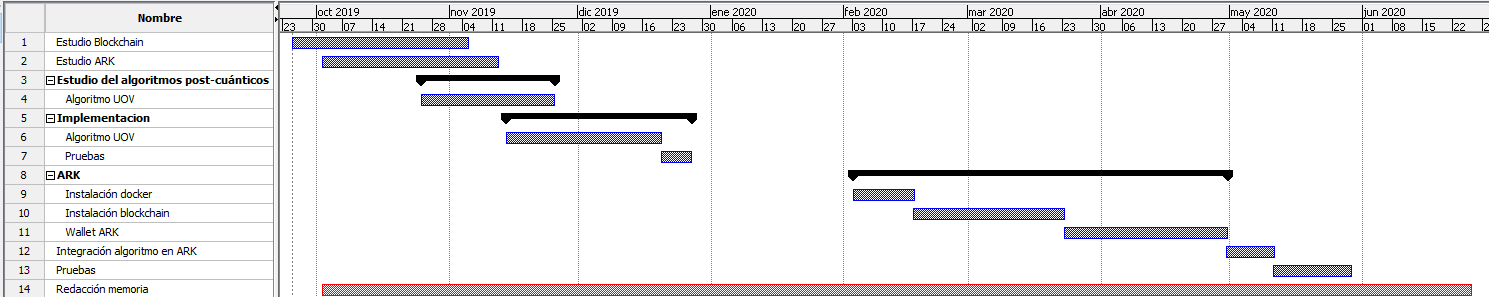
\includegraphics[width=14cm,height=5.5cm]{figuras/Gantt_ini.png}
	\caption{Digrama de Gantt inicial}
	\label{fig:gantt-ini}
\end{figure}

Pero no todo ha sido como se había planificado, puesto que han surgido algunos imprevistos. A la hora de realizar la implementación del algoritmo UOV en \texttt{python} no existe una biblioteca para trabajar con matrices y cuerpos finitos al mismo tiempo, así ha aumentado el tiempo que se iba a dedicar al algoritmo. Además el trabajo con ARK ha sido más tedioso del esperado, retrasando los tiempos programados. El diagrama de Gantt real se ha divido en parte para que se visualice mejor, la imagen \ref{fig:gantt-real-1} muestra las fases de estudio e implementación, la imagen \ref{fig:gantt-real-2} incluye el tiempo dedicado al trabajo con ARK hasta julio y la imagen \ref{fig:gantt-real-3} desde julio hasta noviembre, además del periodo de pruebas.\\


\begin{figure}[h]
	\centering
	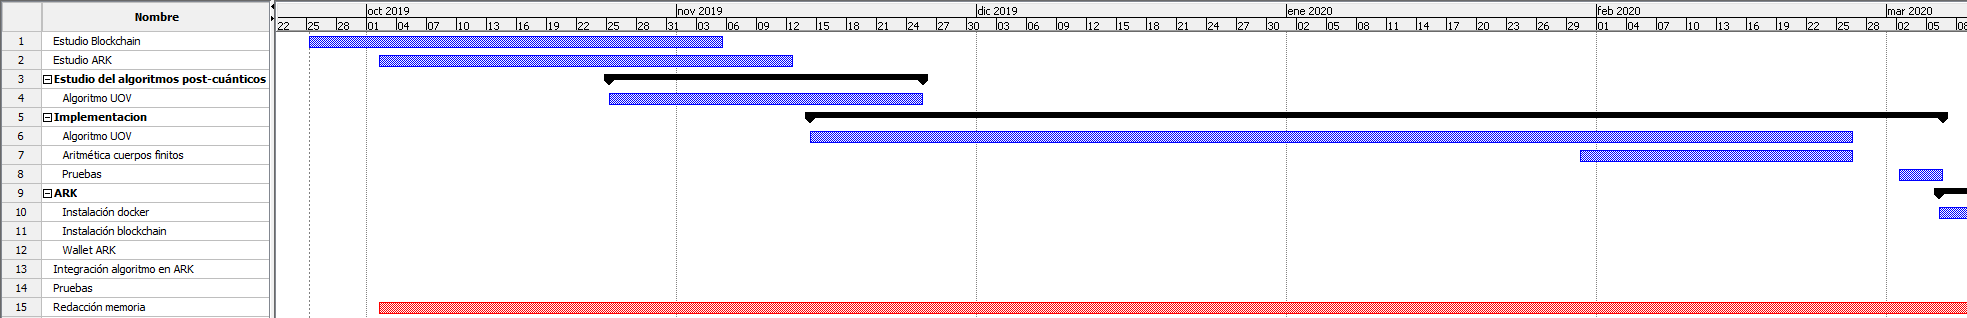
\includegraphics[width=15cm,height=6cm]{figuras/Gantt_1.png}
	\caption{Diagrama de Gantt real. Parte I}
	\label{fig:gantt-real-1}
\end{figure}

\begin{figure}[h]
	\centering
	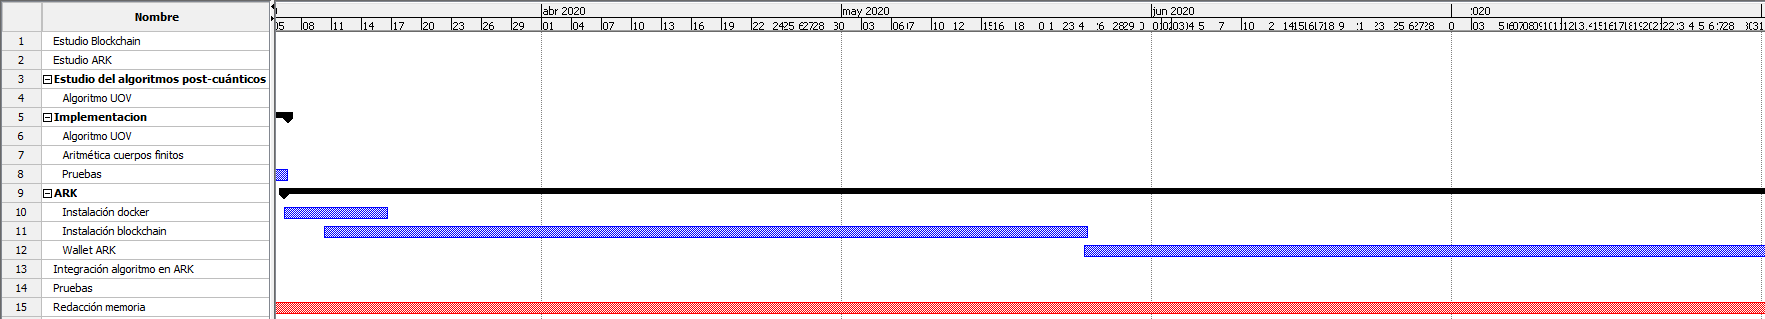
\includegraphics[width=15cm,height=6cm]{figuras/Gantt_2.png}
	\caption{Diagrama de Gantt real. Parte II}
	\label{fig:gantt-real-2}
\end{figure}

\begin{figure}[h]
	\centering
	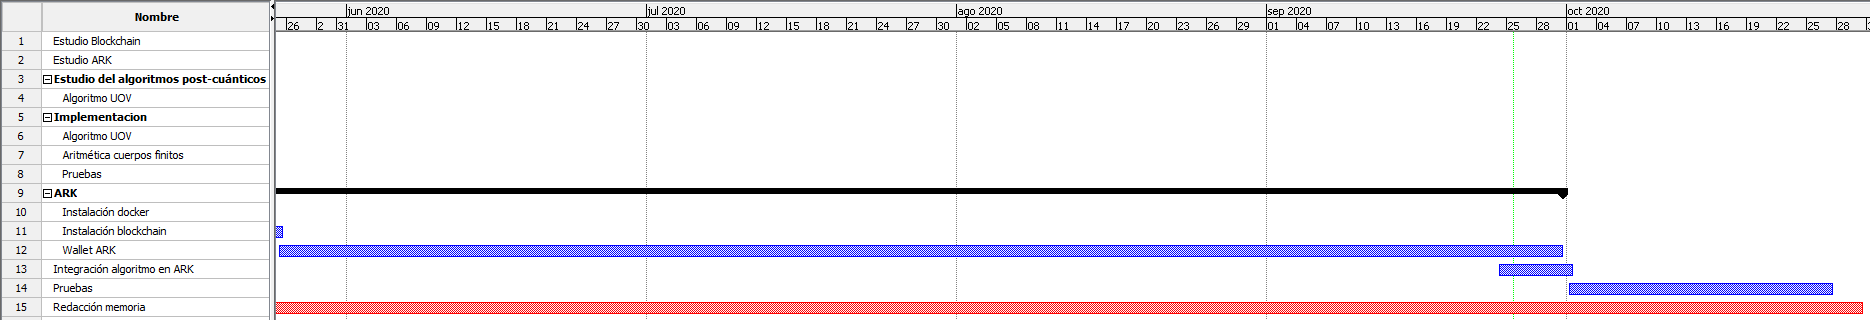
\includegraphics[width=15cm,height=6cm]{figuras/Gantt_3.png}
	\caption{Diagrama de Gantt real. Parte III}
	\label{fig:gantt-real-3}
\end{figure}

\section{Costes}